\chapter{Fundamental Concepts Underlying Neural Networks}
\label{cha:fundanemtalConcepts}

%---------------------------------------------------------------------------

This thesis begins by introducing theory related to neural networks which derive their name from the networks of biological neurons present in our brains. However, although airplanes draw inspiration from birds, they do not need to flap their wings. Similarly, even though neural networks are derived from biological neurons, they became quite different from their biological equivalent, so many scientists believe that this analogy should be abandoned. The reason is to avoid constraining our creativity to structures that can only exist in nature and to open up the potential for more innovative designs that exceed natural limitations~\cite{UMzUSLiTF}.

\section{Perceptrons}

Neural networks consist of \textit{perceptrons} (artificial neurons) which are interconnected to form a more complex structure. To fully understand how neural networks work, it is essential to explain the function of a single perceptron first.

In 1957, Frank Rosenblatt proposed the perceptron, which is the simplest form of an artificial neural network. It is based on an artificial neuron known as a \textit{Threshold Logic Unit} or \textit{TLU}~\cite{UMzUSLiTF}.

\begin{figure}[!htb]
    \centering
    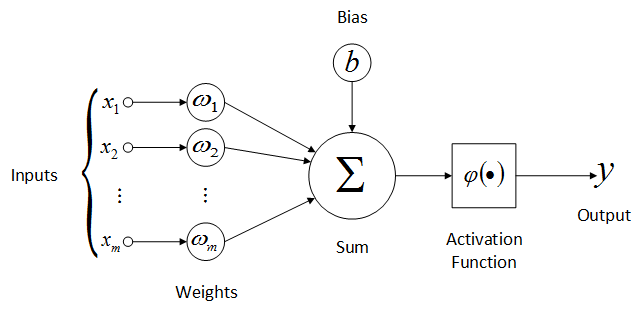
\includegraphics[scale=0.6]{Images/perceprton-model.png}
    \caption{Perceptron model~\cite{PerceptronModel}.}
    \label{fig:perceptronModel}
\end{figure}

The diagram in Figure \ref{fig:perceptronModel} illustrates the structure of a single perceptron, which consists of four essential elements: \textbf{inputs}, \textbf{weights and bias}, a \textbf{summation function}, and an \textbf{activation function}.

The functionality of a perceptron can be described as follows: the inputs and outputs are numerical values, and each connection has assigned a specific weight. The perceptron calculates the sum of the input values each multiplied by their respective weights and adds a bias term to this calculated sum:

\begin{equation}
z = b + \sum_{i=1}^{n} x_iw_i = x^Tw + b
\end{equation}

This weighted sum is then passed through an activation function, which determines the final output value of the perceptron:

\begin{equation}
y = \phi(z)
\end{equation}

A perceptron is composed of a single layer of \textit{TLU} units, with each \textit{TLU} connected to every input. Such a layer is referred to as a fully connected layer. Inputs are fed into artificial neurons, also known as the input layer, whose function is to forward all the received data. Moreover, it is worth mentioning that a perceptron can have more than one output, enabling it to classify samples into multiple categories, therefore functioning as a multi-output classifier~\cite{UMzUSLiTF}~.

Frank Rosenblatt's learning algorithm was inspired by Hebb's rule, which states that when a biological neuron frequently excites another nerve cell, the connection between these neurons becomes stronger. Siegrid Löwel summarized this concept with the phrase: "Cells that fire together, wire together," which loosely translates to "Cells that excite each other tend to connect more strongly." This means that the connection weight between two neurons tends to increase when they are activated at the same time.

Perceptrons use a variant of this rule during training, taking into account the error the network makes during outcome predictions. This means that connections that help reduce the error value are strengthened. More specifically, the perceptron processes one training example at a time and calculates predictions for each. For each output neuron responsible for an incorrect result, the weights of connections from all inputs contributing to the correct prediction are increased. 

The equation \ref{eq:weightsUpdate} represents the process of updating weights in perceptron learning:

\begin{equation}
    w_{i,j}^{k + 1} = w_{i,j}^k + \eta(y_j - \bar{y}_j)x_i
    \label{eq:weightsUpdate}
\end{equation}

where:
\begin{eqwhere}[2cm]
\item[$w_{i,j}$] is the weight of the connection between the i-th input and the j-th output neuron
\item[$x_i$] is the i-th input value of the current training example
\item[$\bar{y}_j$] is the output of the j-th output neuron for the current training example
\item[$y_j$] is the expected output of the j-th output neuron for the current training example
\item[$\eta$] is the learning rate
\item[$k$] is the step
\end{eqwhere}

It is worth noting that Rosenblatt proved that the learning algorithm will converge if the training samples are linearly separable. A concept was formalized in the perceptron convergence theorem~\cite{UMzUSLiTF}.

\section{Deep Neural Networks}

In their simplest form, perceptrons have several significant drawbacks. Marvin Minsky and Seymour Papert pointed out some of these limitations in their 1969 monograph, "Perceptrons"~\cite{PerceptronsBook}. For instance, the perceptron cannot solve trivial problems, such as the exclusive OR (XOR) classification task. However, researchers have discovered that many of these limitations can be overcome by creating multiple layers of perceptrons. 

A \textit{Multi-Layer Perceptron} (\textit{MLP}) consists of one input layer, at least one hidden layer of Threshold Logic Units (TLUs), and a final output layer. This architecture enables the MLP to tackle problems that a single-layer perceptron cannot, including the XOR problem.

\begin{figure}[!htb]
    \centering
    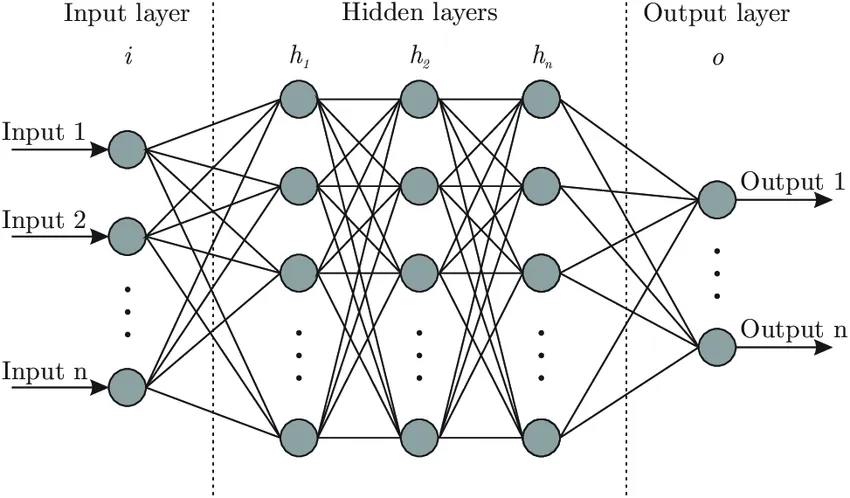
\includegraphics[scale=0.5]{Images/nn_model.jpg}
    \caption{Neural network model~\cite{NNModel}.}
    \label{fig:NNModel}
\end{figure}

An artificial neural network is called a \textit{Deep Neural Network (DNN)} if it contains multiple hidden layers. It is noteworthy that the term "deep" is quite relative - it can imply anything from a few to over a hundred hidden layers. Layers located close to the output layer are called upper layers, while those closer to the input layer are known as lower layers. Each layer includes a bias neuron and is fully connected to the subsequent layer.

For decades, scientists have been searching for an effective way to train deep neural networks. The breakthrough arrived in 1986 with the introduction of the \textbf{backpropagation algorithm} by David Rumelhart, Geoffrey Hinton, and Ronald Williams~\cite{UMzUSLiTF}.

The backpropagation algorithm leverages the gradient descent algorithm. By utilizing automatic differentiation to calculate gradients, backpropagation can evaluate the error gradient for each model parameter in just two passes, forward and backward. This process determines the degree to which all connection weights and biases should be modified to reduce error. Once these gradients are obtained, the classic gradient descent algorithm updates the weights and biases, continuing until a maximum number of iterations is reached. Taking a closer look at the next steps of the backpropagation algorithm:


\begin{enumerate}
    \item The algorithm starts with a \textbf{forward pass} where results for all neurons are calculated and passed on, retaining intermediate outcomes for later use.
    \item The network's \textbf{output error is measured} using a formula, which involves squaring the difference between the expected and actual outcomes and multiplying by a half coefficient to simplify the differentiation process:
    \begin{equation*}
            \epsilon = \sum \frac{1}{2} (y_{o} - y_{u})^2
    \end{equation*}
    \item The \textbf{backward pass} calculates gradients for each weight and bias which minimizes the error calculated in the previous step. This involves calculating, via the chain rule, how each output connection contributes to the error. This process starts from the last hidden layer, assessing the impact of each weight on the outcome, and repeats for preceding layers, returning to the input layer.
    \item The final step involves applying \textbf{gradient descent} to update all the network's weights using the gradients calculated in the previous step.
\end{enumerate}
 
For deep neural networks, the amount of data used can be huge. In such a case, the data is divided into smaller groups called \textit{\textbf{batches}}. For instance, a batch can contain $32$ training instances. Each run of the algorithm is called an \textit{\textbf{epoch}}.

\subsection{Activation Functions}

Activation functions introduce non-linearity to neural networks, which enables them to solve complex problems that cannot be solved by linear transformations alone. Without activation functions, any deep network could essentially be simplified to a single-layer network, regardless of its depth - when multiple linear functions are combined using a linear transformation, another linear function is obtained. Activation functions such as the logistic (sigmoid) function, ReLU, and tanh allow networks to approximate any continuous function, which significantly enhances their computational power and ability to handle intricate tasks~\cite{ActivationFunctions}. Examples of activation functions are shown in the Figure \ref{fig:activFun}.

\begin{figure}[!htb]
    \centering
    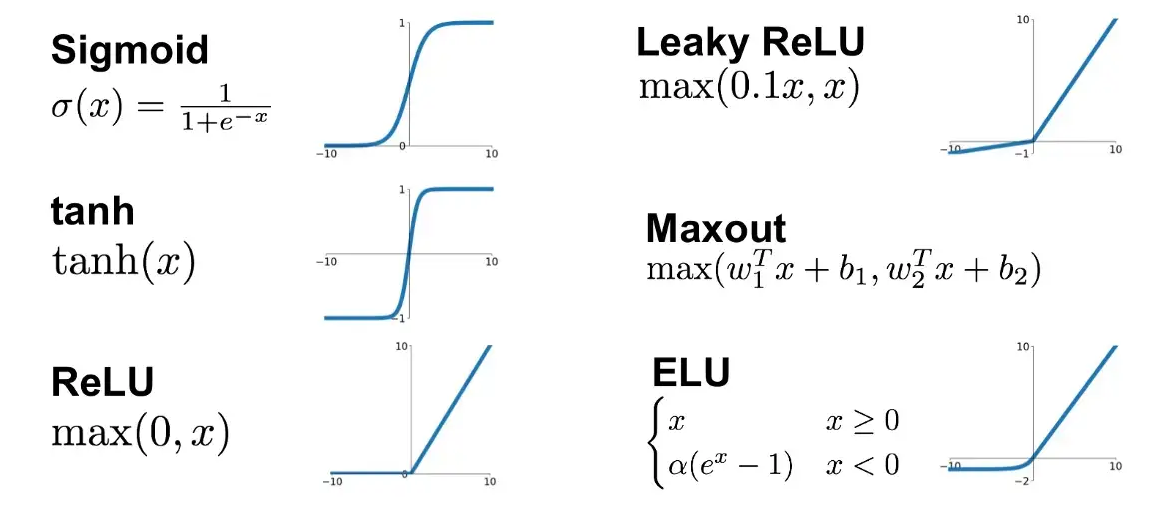
\includegraphics[scale=0.4]{Images/activation-functions.png}
    \caption{Activation functions examples~\cite{ActivationFunctionsImage}.}
    \label{fig:activFun}
\end{figure}

%---------------------------------------------------------------------------

\subsection{Limitations of the MLP Model in Image Processing}
\label{ssec:MLPLimitations}

Traditional multilayer neural networks face challenges when processing images, as highlighted in~\cite{TDS-NNCons}. One major issue is that Multilayer Perceptron (MLP) networks require \textbf{one input perceptron per image pixel} for grayscale images, and for RGB images,  each pixel needs three input perceptrons, leading to three weights per pixel that need to be calculated and stored. This means that for a $224$x$224$ RGB image, over $150,000$ weights need updating, which can significantly increase training time and the risk of overfitting. Overfitting occurs when the network performs well on training data but poorly on new, unseen data.

Additionally, MLP networks struggle when dealing with input images that are \textbf{shifted} or \textbf{rotated}, or when the object of interest appears in \textbf{different locations} across images. For instance, if an object is mostly located in the top left corner in the training data, the network may learn to only recognize objects in that specific part of an image, leading to misclassification when the object appears elsewhere. This problem arises because the network emphasizes connections corresponding to the pixels where the object is most frequently observed.

Another drawback of MLP networks is the loss of \textbf{spatial information} when an image is flattened for MLP model input. Neurons close to each other capture certain image features, making it crucial to preserve spatial information to teach the model to recognize objects regardless of their position in the image. Traditional multilayer neural networks lack this capability, failing to utilize pixel adjacency to identify features that could later be used for object recognition.

%---------------------------------------------------------------------------

\section{Convolutional Neural Networks}
\label{sec:CNNs}

Given that the data used in this research consists of images, this subsection will introduce \textit{Convolutional Neural Networks} (\textit{CNNs}) - a popular type of neural network utilized in image data analysis. CNN's name comes from convolution, which is the main operation used for image feature extraction.

\begin{figure}[!htb]
    \centering
    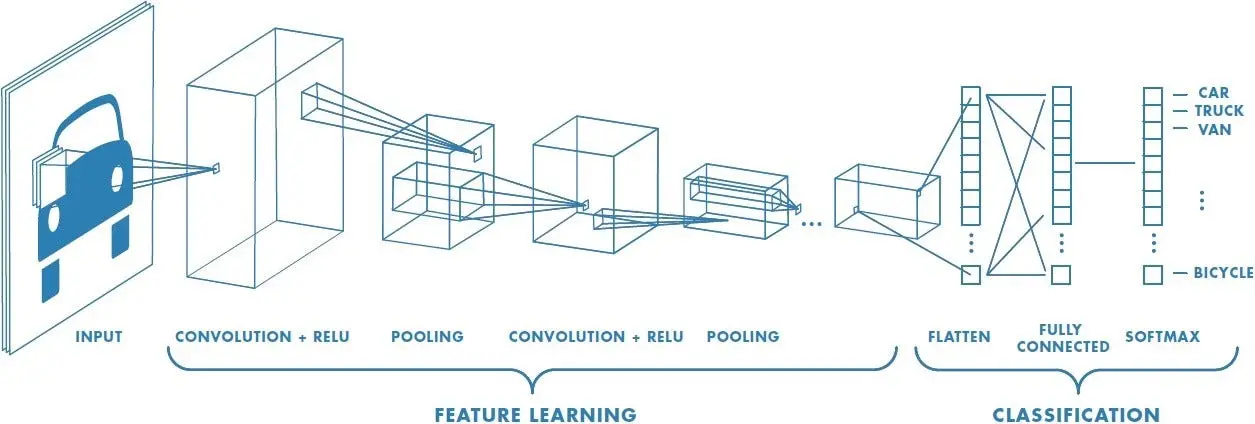
\includegraphics[scale=0.3]{Images/CNN-model.jpg}
    \caption{Convolutional Neural Network~\cite{CNNBlogGuide}.}
    \label{fig:CNNModel}
\end{figure}

Convolutional neural networks allow you to analyze images using \textbf{feature extraction} and \textbf{pattern recognition}. The operation of CNNs can be broken down into the following steps:

\begin{enumerate}
    \item   Initially, \textit{\textbf{image padding}} adds a frame of pixels around the input image, ensuring the dimensions remain the same after convolution.
    \item   A \textit{\textbf{filter}} (usually $3x3$ or $5x5$) detects specific shapes in the input image through \textit{\textbf{convolution}}. It multiplies each pixel in a region by corresponding filter values and sums the results, moving across the image to create \textit{feature maps}. The filter parameters determine the number of feature maps, highlighting areas where the feature is present.
    
    The weight values in filters are calculated automatically, meaning the distinctive features of the objects under analysis are determined during the learning process of the convolutional network.
    \item   Next, \textit{\textbf{activation functions}} are used to remove insignificant information from the feature maps, which speeds up network training by setting negative values (indicating the absence of sought-after features in a given area) to zero or another small value.
    \item   The following step involves \textit{\textbf{pooling}}, with \textit{\textbf{max pooling}} being the most common variant. This involves traversing the feature map with a window and selecting the pixel with the highest value from each neighborhood. For \textit{\textbf{average pooling}}, the average value is used. This value is then used to replace the entire area. This reduces the feature map size while retaining important information.
    \item   The processes of \textit{\textbf{convolution}} and \textit{\textbf{pooling}} are then alternated according to the network's architecture. Each subsequent layer identifies more abstract features. For example, in a plant species recognition network, early layers detect basic elements like edges and textures, while later layers identify detailed attributes such as leaf shape, vein patterns, and the presence of flowers or fruits. Advanced layers integrate these details to distinguish between species, focusing on specific characteristics like leaf shape, flower color, and growth habits.
    \item Finally, the last layer of the convolutional network is \textbf{\textit{fully connected}} and is responsible for the final classification. The input to this layer is flattened from matrices into a vector.
\end{enumerate}

Considering the limitations outlined in section \ref{ssec:MLPLimitations}, it is clear that traditional multilayer neural networks face notable challenges, especially in the context of image processing. Convolutional Neural Networks (CNNs) effectively address these limitations. To illustrate this advancement, each stage of a CNN is analyzed. A detailed analysis showing how each stage directly addresses these limitations is presented in Table \ref{tab:CNNStages}.

It is essential to keep in mind that Convolutional Neural Networks (CNNs), despite their advanced capabilities, \textbf{demand a wide spectrum of training examples} to achieve optimal performance. In cases where the variability among examples is limited, employing \textbf{data augmentation becomes crucial}. This technique is the core of the analysis in this master's thesis. It enables the generation of a diverse set of samples, ensuring that the CNN is well-equipped to handle various scenarios in image analysis.

\begin{table}[H]
    
    \caption{Applications and Functions of Convolutional Network Stages.}
    \centering
    \begin{tabular}{|>{\centering\arraybackslash}m{4cm}|>{\centering\arraybackslash}m{3.9cm}|>{\centering\arraybackslash}m{6.8cm}|}
     
      \hline
     \textbf{Stage} & \textbf{Function} & \textbf{Application}  \\ 
      \hline
      Convolution & Using a filter extracts the features of the object visible in the image. & Enables sparser connections.
      
      Reduces the number of parameters.
      
      Prevents overfitting.
      
      Combined with pooling, it ensures the target object's position in the image does not affect classification.\\ 
      \hline
      Activation Function & Introduces non-linearity. & Improves training and prediction speed. \\

      \hline
      Pooling & Replaces a neighborhood of pixels with a singular value. & Reduces dimensionality. 
      
      Increases robustness to distortions and variability in images as the arrangement of values within the neighborhood becomes irrelevant.\\
      \hline
      Classification & Utilizes a fully connected layer of neurons to predict the final outcome. & Facilitates the recognition of objects that are distinct yet represent the same category, enhancing the network's resilience to a wide array of test cases.\\
      \hline
    
    \end{tabular}
    \label{tab:CNNStages}
\end{table}

%---------------------------------------------------------------------------

\section{Generative Adversarial Networks (GANs)}
\label{sec:GANs}

Generative Adversarial Networks (GANs) are one of the most significant advancements in artificial intelligence and machine learning in the last decade. This chapter explores the foundational concepts, mechanisms, and applications of GANs, which have revolutionized generative modeling and opened new possibilities in areas such as image generation, video synthesis, and more.
%---------------------------------------------------------------------------

\subsection{Introduction to GANs}

Generative Adversarial Networks (GANs) were introduced by Ian Goodfellow et al in 2014~\cite{GANsOriginalPaper}. GAN consists of two distinct models: a \textbf{generator} and a \textbf{discriminator}. These models are trained simultaneously in a zero-sum game framework, where the generator aims to produce realistic data instances, and the discriminator attempts to distinguish between real and generated data. The adversarial nature of this framework drives both models to improve continuously.

In most GAN architectures, both the generator and discriminator consist mainly of convolutional and fully connected layers. The generator is a mapping between a vector of random values (called the latent space) to the space of data (images in our case): $\mathcal{G}: \mathcal{G}(z) \rightarrow \mathcal{R}^{|x|}$ where $z \in \mathbb{R}^{|z|}$ is a sample from the latent space, $x \in \mathbb{R}^{|x|}$ is an image and $| \cdot |$ denotes the number of dimensions. On the other hand, the discriminator may be characterized as a function that maps from image data to a probability that the image comes from the real data distribution. It can be represented as follows: $\mathcal{D}: \mathcal{D}(x) \rightarrow (0, 1)$.

\begin{figure}[!htb]
    \centering
    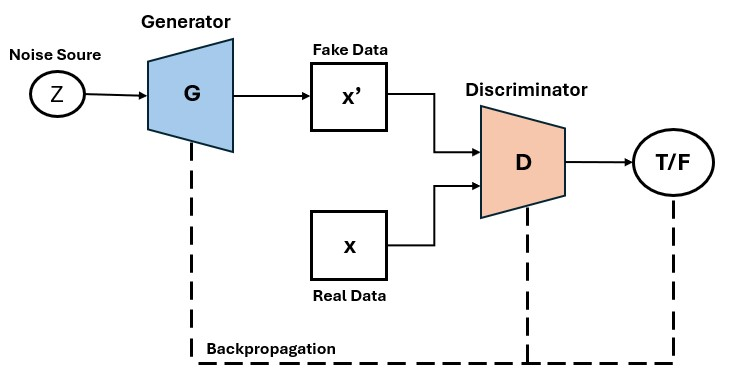
\includegraphics[scale=0.5]{Images/gan_framework.jpg}
    \caption{GAN framework. Inspired by~\cite{GANFramework}.}
    \label{fig:GANFramework}
\end{figure}

As shown in Figure \ref{fig:GANFramework}, the generator does not have direct access to real images. The only way it can learn the high-dimensional distribution behind the data is through interaction with the discriminator which can access both synthetic and real samples. The error signal, derived from a straightforward comparison with the ground truth, can be used to train both the generator and discriminator. By backpropagating this error, the discriminator's ability to classify images improves, and at the same time, the generator's capability to produce higher-quality images is enhanced. Once we are satisfied with the effectiveness of the discriminator, we can stop training it and continue to train only the generator. 
If the distribution created by the generator perfectly aligns with the actual data distribution, then the discriminator should reach its highest level of uncertainty and assign a probability of 0.5 to every input.\cite{GANOverview} The training of GANs is discussed in detail in section \ref{ssec:GANsTraining}.

To address specific challenges and improve generative performance, a variety of architectures have been developed. In the domain of data augmentation, Generative Adversarial Networks (GANs) have emerged as powerful tools for generating synthetic data, enhancing the diversity and volume of datasets. Types of GAN models particularly effective in this domain are presented in section \ref{ssec:typesOfGANs}.

% Particularly effective in this domain are Conditional GANs (cGANs), which can produce images conditioned on specific attributes or classes, thereby enriching category-specific data. CycleGANs also play a crucial role by facilitating image-to-image translation tasks without the need for paired examples, allowing for the augmentation of datasets across different styles or domains. Another significant contribution comes from DCGANs (Deep Convolutional GANs), which leverage convolutional neural networks to generate high-quality images that can mimic various real-world variations.

%---------------------------------------------------------------------------
\subsection{GANs Training}
\label{ssec:GANsTraining}

Training of Generative Adversarial Networks is described in detail in~\cite{GANOverview}. The GAN training is a complex and iterative process that involves optimizing two neural networks — the generator and the discriminator — against each other. This process can be described as a game where the generator's goal is to produce data indistinguishable from source data, while the discriminator's goal is to correctly classify data as real or fake.

To achieve this, a value function $V(G,D)$ is used to update the discriminator and generator in a synchronized fashion. This value function depends on the current state of both networks. Training involves solving a min-max optimization problem where the discriminator tries to maximize its ability to distinguish real data from fake, and the generator tries to minimize the discriminator's accuracy. The standard GAN loss function is described by equations \ref{eq:GANOptimization} and \ref{eq:GANLoss}.
    
\begin{equation}
    \max_{D} \min_{G} V(G, D),
    \label{eq:GANOptimization}
\end{equation}

where

\begin{equation}
    V(G, D) = \mathbb{E}_{x}[\log D(x)] + \mathbb{E}_{z}[\log (1 - D(G(z)))]
    \label{eq:GANLoss}
\end{equation}

This loss function of a Generative Adversarial Network (GAN) guides the training of both components of GANs. It consists of two expressions: the first expression (\(\mathbb{E}_{x}[\log D(x)]\)) measures how well the discriminator recognizes actual data, and the second expression (\(\mathbb{E}_{z}[\log (1 - D(G(z)))])\)) measures the discriminator's ability to detect fake data produced by the generator. Together, they form a tug-of-war where the discriminator improves its detection skills while the generator tries to create increasingly convincing fakes. 

Although this function seems to be useful, in practice, it saturates quickly for the generator, which means that it frequently stops training if it does not keep pace with the discriminator. To address this issue, a refined version of the standard GAN loss employs a strategy where the generator aims to maximize $- log(D(G(z))$. This adaptation focuses on increasing the likelihood of generated images being classified as real rather than decreasing their likelihood of being found fake~\cite{GANEquations}.


The standard GAN loss function can be divided into two parts: \textbf{generator loss} and \textbf{discriminator loss}. During training, the discriminator is typically trained first in each cycle. It is updated to maximize its accuracy on identifying real versus generated data. This is done by feeding it real data and training it to predict ‘real’, and then feeding it fake data from the generator and training it to predict ‘fake’. This step is crucial because a well-trained discriminator guides the generator toward producing more realistic data. The discriminator punishes itself for wrongly identifying a real instance as false, or a false instance (made by the generator) as true, through the maximization of the following function \ref{eq:discrimnator}.

\begin{equation}
    \nabla_{\theta_d} \frac{1}{m} \sum_{i=1}^{m} \left[ \log D \left( x^{(i)} \right) + \log \left(1 - D \left( G \left( z^{(i)} \right)\right)\right) \right]
    \label{eq:discrimnator}
\end{equation}

Subsequently, the generator is updated. It aims to produce data that the current discriminator will classify as real. This is achieved by modifying the generator's parameters in a way that minimizes the output of the discriminator. Ideally, the discriminator should reach a point where it predicts 0.5 for all inputs, indicating it is unable to distinguish between real and fake data. This state indicates that the generator produces highly realistic data. To train the generator, the function in equation \ref{eq:generator} must be minimized. The generator gets rewarded for successfully fooling the discriminator and gets penalized otherwise. 

\begin{equation}
    \nabla_{\theta_g} \frac{1}{m} \sum_{i=1}^{m} \log \left(1 - D \left( G \left( z^{(i)} \right)\right)\right)
    \label{eq:generator}
\end{equation}

However, training GANs can be unstable, and convergence is not always guaranteed. The networks may end up in a situation where the generator produces a limited range of outputs, or the discriminator may become too effective too quickly, leaving the generator with no meaningful gradient to learn from. To address these issues, techniques such as \textbf{feature matching} and \textbf{minibatch discrimination} have been proposed. These methods stabilize the training process by ensuring that the generator produces diverse outputs, and the discriminator evaluates batches of data instead of individual samples~\cite{GANOverview}.


\begin{figure}[!htb]
    \centering
    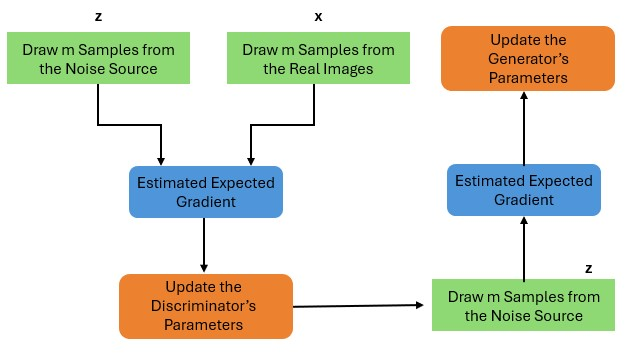
\includegraphics[scale=0.65]{Images/gan-training.jpg}
    \caption{GANs training. Inspired by~\cite{GANOverview}.}
    \label{fig:GANTraining}
\end{figure}

\subsection{Types of GANs}
\label{ssec:typesOfGANs}

This section explores several main types of Generative Adversarial Networks (GANs), each serving distinct purposes and exhibiting unique characteristics. The information presented here is based on an article that provides an overview of GANs~\cite{GANOverview}.

\textbf{Standard GANs}: First, we have Standard GANs. These initial GAN architectures used fully connected neural networks for both the generator and discriminator. Standard GANs were applied to simpler datasets like MNIST, CIFAR-10, and the Toronto Face Dataset, and they set the foundation for more complex models.

\textbf{Deep Convolutional Generative Adversarial Networks (DCGANs)}: DCGANs were introduced to bridge the gap between the success of Convolutional Neural Networks (CNNs) in supervised learning (mentioned in Section \ref{sec:CNNs}) and their potential in unsupervised learning. The original DCGAN paper~\cite{OriginalDCGAN} detailed how DCGANs apply CNN architectures shown in Figure \ref{fig:DCGANsFlow}, which are successful in tasks like image classification, to the generative model of GANs. This allows for robust learning of \textbf{feature hierarchies} and more detailed and nuanced image generation.


\begin{figure}[!htb]
    \centering
    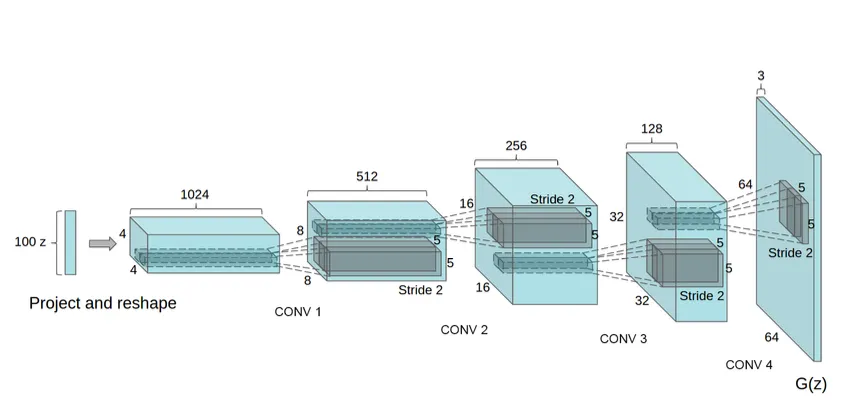
\includegraphics[scale=0.4]{Images/DCGAN-example.jpg}
    \caption{DCGANs flow~\cite{DCGANsFlow}.}
    \label{fig:DCGANsFlow}
\end{figure}

Additionally, DCGANs propose several key architectural innovations to promote stable training of GANs, particularly for generating high-resolution images. These innovations include:
\begin{enumerate}
    \item \textbf{Replacing Pooling Layers}: DCGANs replace pooling layers with strided convolutions in the discriminator and fractional-strided convolutions in the generator. This helps the networks learn their own spatial hierarchies.
    \item \textbf{Using Batch Normalization}: This technique is applied across the entire network, with the exception of the generator's output layer and the discriminator's input layer. It standardizes the inputs to each unit, mitigating the internal covariate shift problem and stabilizing training dynamics.
    \item \textbf{Eliminating Fully Connected Layers}: DCGANs suggest removing fully connected hidden layers to rely entirely on convolutional layers to improve training and reduce the risk of overfitting.
    \item \textbf{Activation Functions}: The generator uses the ReLU activation function in all layers except for the output, which uses the Tanh function. This encourages the model to learn faster and cover the color space more effectively. The discriminator employs the LeakyReLU activation for better gradient flow, especially beneficial when dealing with higher-resolution images.
\end{enumerate}

\textbf{Conditional Generative Adversarial Networks (cGANs)}: cGANs are a type of GANs that are specifically designed to generate output data in a \textbf{controlled manner}. Unlike standard GANs that generate data without a specific direction, cGANs utilize additional label information to guide the generation process. This involves modifying both the generator and discriminator to accept label data (y), allowing the network to condition its outputs on these labels. The mathematical framework of cGANs extends the standard GAN formula by incorporating conditional probabilities, which align the generated outputs with predefined labels. This mechanism not only accelerates the convergence of the network but also allows for control over the characteristics of the generated images at testing time, making cGANs highly effective for tasks requiring specified outputs, such as data augmentation~\cite{cGANs}. You can refer to Figure \ref{fig:cGANsFramework} for a better understanding of the cGANs framework. The cGANs framework is useful for tasks that require generating targeted data outputs.

\begin{figure}[!htb]
    \centering
    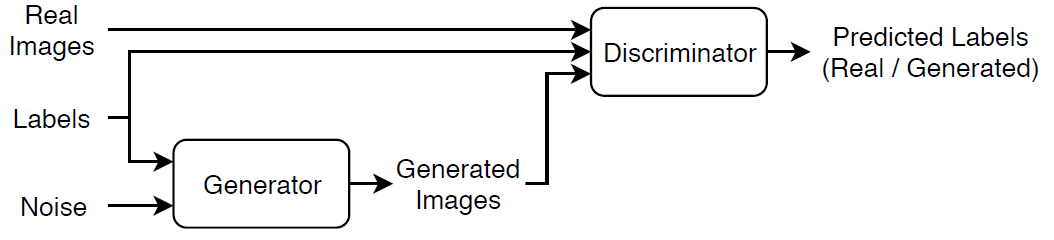
\includegraphics[scale=0.35]{Images/cgan-diagram.png}
    \caption{Conditional GANs framework~\cite{cGANs}.}
    \label{fig:cGANsFramework}
\end{figure}

\textbf{CycleGAN}: CycleGANs are a type of neural network that can perform image-to-image translation without the need for paired examples. This is achieved through the use of two generators and two discriminators that work together to map images from one domain to another. What makes CycleGANs stand out is the incorporation of Cycle Consistency Loss, which ensures that an image converted from one domain back to its original domain retains its original features. This means that transformations, such as turning a horse into a zebra (Figure \ref{fig:cycleGANsExample}), can be reversed. CycleGANs are ideal for tasks without paired training data, marking a significant advance in unsupervised learning~\cite{cycleGANs}.

\begin{figure}[!htb]
    \centering
    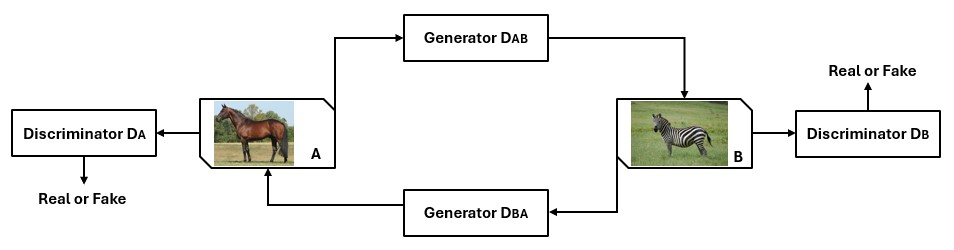
\includegraphics[scale=0.62]{Images/cycleGANexample.jpg}
    \caption{CycleGANs example described in this section. Based on~\cite{cycleGANs}.}
    \label{fig:cycleGANsExample}
\end{figure}

\textbf{StyleGANs}: StyleGANs, developed by NVIDIA, are explained in detail in this article~\cite{StyleGAN}. They integrate and extend the progressive training methodology of ProGAN~\cite{ProGAN}. This methodology scales up image resolution from lower to higher during the training process, which enhances stability and image quality throughout the training phase. 

StyleGANs have a style-based generator that separates high-level attributes (like pose and identity) from stochastic variations (like skin texture or hair details) within images. This separation is achieved through an intermediate latent space that allows the manipulation of styles at different levels of the synthesis network, using a technique called Adaptive Instance Normalization (AdaIN). Each level of detail, from coarse to fine, can be adjusted independently without affecting other levels. This provides unprecedented control over the synthesis process.

\begin{figure}[!htb]
    \centering
    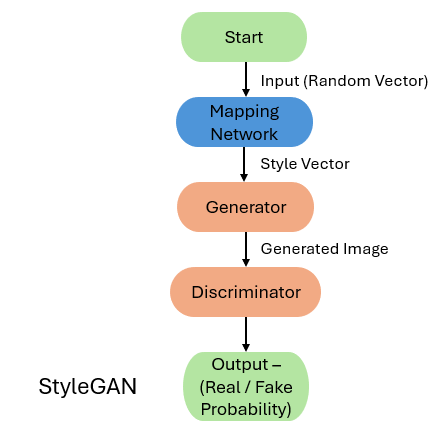
\includegraphics[scale=0.63]{Images/style-gan-high-level.png}
    \caption{StyleGAN - High-Level overview. Inspired by~\cite{StyleGANHighLevel}.}
    \label{fig:styleGANHighLevel}
\end{figure}

Moreover, StyleGAN enhances feature control through a mapping network that converts input vectors into an intermediate latent space. This space more effectively disentangles factors of variation, allowing for easier manipulation of individual features without affecting others. This capability makes StyleGAN not only a powerful tool for generating highly realistic images but also improves its ability to perform targeted modifications and explorations of the generative space. A high-level overview of StyleGAN's functionality is visualized in Figure \ref{fig:styleGANHighLevel}.

The features of StyleGAN technology have placed it at the forefront of GAN technology. It has pushed the limits of how artificial images can be refined and controlled for tasks that require high levels of detail and realism. The model's ability to generate nuanced, customizable images has broad implications for fields ranging from digital content creation to training data enhancement for machine learning algorithms. Examples of images generated by StyleGAN are shown in Figure \ref{fig:styleGANExample}.

\begin{figure}[!htb]
    \centering
    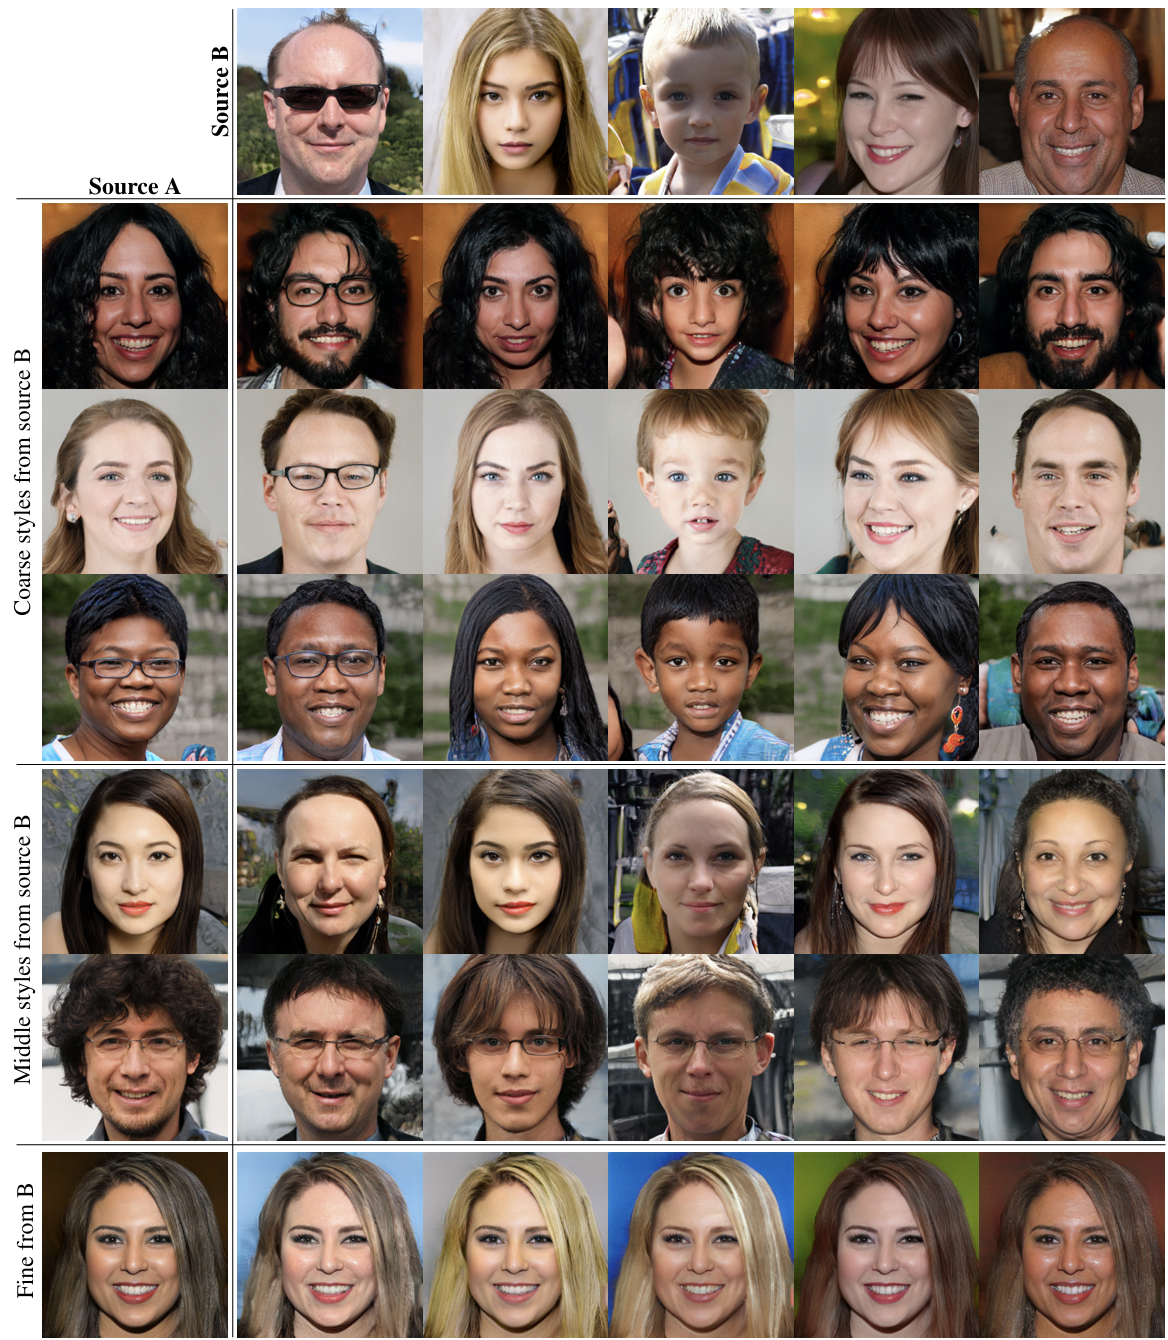
\includegraphics[scale=0.6]{Images/style-gan-example.png}
    \caption{Examples of images created by StyleGAN. Images were generated from two latent spaces: Source A and B. A particular subset of styles was then transferred from Source B to Source A. Depending on the resolution of the styles transferred, different degrees of change were achieved in the images. When coarse styles were copied from Source B to A, the gender and age of the images were preserved. If middle-resolution styles were transferred, smaller facial features, hairstyles, and eye openness from Source B were inherited by the images from Source A. However, the general face shape, pose, and eyeglasses from Source A were still preserved. For fine-grained styles, only minor changes such as hair color were applied~\cite{cycleGANs}.}
    \label{fig:styleGANExample}
\end{figure}

%---------------------------------------------------------------------------

\section{Transfer Learning}
\label{sec:transferLearning}
Transfer learning was first introduced by Stevo Bozinovski in 1976, with the original article written in Croatian. In 2020, a follow-up article was published, providing a detailed mathematical and geometric theory related to transfer learning~\cite{TransferLearningFirst}.

This subsection draws insights from the book~\cite{TransferLearning}, which extensively explores both the theoretical aspects and practical implementations of transfer learning, particularly using the Python programming language. The aim is to provide a comprehensive discussion on the topic.

The core concept of transfer learning, illustrated in Figure \ref{fig:transferLearning}, is based on the principle of leveraging existing knowledge to master new tasks. It is similar to learning a new language - if you are proficient in Spanish, you will find it easier to learn Portuguese due to the similarities between the two languages. Similarly, we can take advantage of established network architectures (like \textit{EfficientNet}), which have been previously trained on vast datasets. This approach is beneficial because the initial layers of convolutional networks are trained to identify simple visual features. By modifying the architecture's last few layers with new, adjustable parameters aimed at recognizing more complex features specific to a new task, we can rapidly create an effective neural network.

\begin{figure}[!htb]
    \centering
    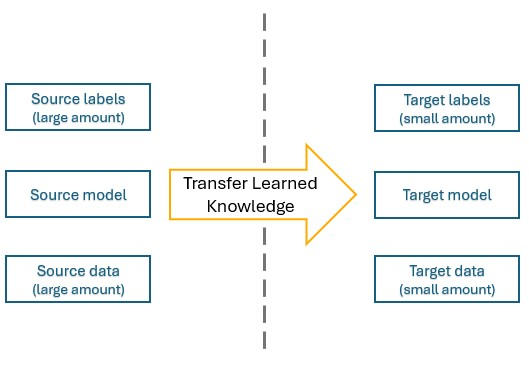
\includegraphics[scale=0.8]{Images/transfer-learning.jpeg}
    \caption{Idea behind transfer learning~\cite{TransferLearningExample}.}
    \label{fig:transferLearning}
\end{figure}

Initially, a well-known model trained on a comprehensive dataset is selected. In the case of images, the ImageNet dataset is often used. It includes around 14 million images, categorized into more than 20,000 categories. The next step is to decide which of the trained weights to freeze, preventing their values from changing. Typically, initial layers weights from the base model are frozen to accelerate the learning process. The next phase involves appending a new model on top of the pre-trained network. The weights of this new model are not fixed but are instead fine-tuned to address the specific characteristics of our dataset. This results in a strong multi-layered model with minimal time investment.

%---------------------------------------------------------------------------

\section{Pre-trained Models}
\label{sec:pretrainedModels}

%---------------------------------------------------------------------------

\subsection{ResNet}

Introduced in 2015, the \textit{ResNet} architecture (short for \textit{Residual Networks}) is detailed in the study~\cite{DeepResidualLearning} by \textit{Kaiming He et al.}, which serves as a key reference throughout this subsection. The developers of this technique identified that a more efficient strategy than extending successive identity connections is to skip over a few connections while assigning near-zero values to filters and then aggregating the results of these processes, as illustrated in Figure \ref{fig:resNetSkipConnections}. This technique enables the emulation of the identity function, which helps to avoid the vanishing gradient problem when necessary.

\begin{figure}[!htb]
    \centering
    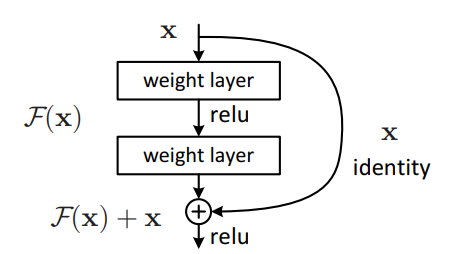
\includegraphics[scale=0.5]{Images/skip-connection.png}
    \caption{Skip-connections~\cite{DeepResidualLearning}.}
    \label{fig:resNetSkipConnections}
\end{figure}

The \textit{ResNet} network is designed with residual connections every few layers. Figure \ref{fig:CNNcomparision} compares the architecture of the \textit{VGG-19} network, a standard 34-layer convolutional network, and a 34-layer residual network.

\begin{figure}[!htb]
    \centering
    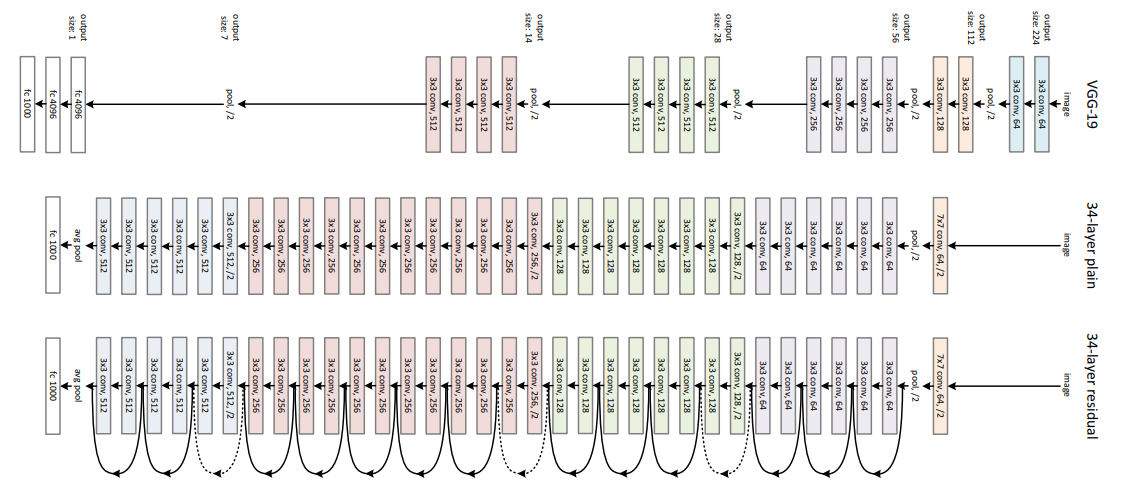
\includegraphics[scale=0.4]{Images/34-layers-nets-comparision.png}
    \caption{CNN architectures comprasion~\cite{DeepResidualLearning}.}
    \label{fig:CNNcomparision}
\end{figure}

The use of residual connections allows for building deeper architectures without vanishing gradient problems (Figure \ref{fig:ResNetLearningCurves}). Notably, even though \textit{ResNet} networks can have up to 152 layers, they are less complex than \textit{VGG} networks with 19 layers due to the implementation of residual connections. Specifically, \textit{ResNet-152} performs approximately $11.3$ billion addition/multiplication operations, whereas \textit{VGG-19} requires about $19.6$ billion operations.

\begin{figure}[!htb]
    \centering
    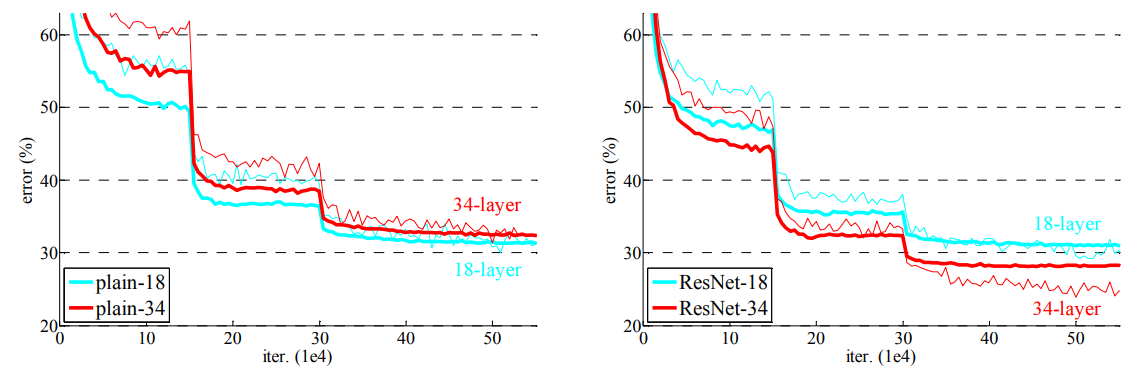
\includegraphics[scale=0.5]{Images/res-net-learning-curves.png}
    \caption{Comparison of learning curves of simple and residual networks~\cite{DeepResidualLearning}.}
    \label{fig:ResNetLearningCurves}
\end{figure}


In conclusion, as more layers are added, \textit{ResNet} networks demonstrate improved performance until overfitting occurs. The effectiveness of residual connections increases with the network's depth. For \textit{ResNet} architectures with more than 34 layers, special structures known as \textit{bottleneck} designs are commonly employed to enhance computational efficiency, as illustrated in Figure \ref{fig:bottleNeck}. These designs consist of three layers: a dimension-reducing layer (1x1 filter), a feature-detecting layer (3x3 filter), and a dimension-restoring layer (1x1 filter). This arrangement allows the feature-detecting layer to operate on a reduced dimensionality, thereby speeding up the computational process.

\begin{figure}[!htb]
    \centering
    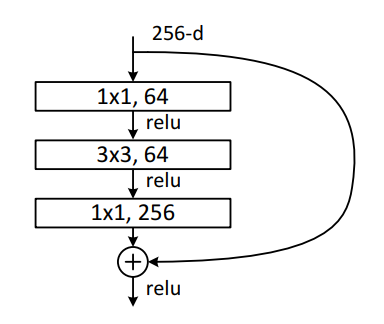
\includegraphics[scale=0.5]{Images/bottle-neck.png}
    \caption{Bottle-neck structure used in \textit{ResNet} networks~\cite{DeepResidualLearning}.}
    \label{fig:bottleNeck}
\end{figure}

%---------------------------------------------------------------------------

\subsection{EfficientNet}

The paper "EfficientNet: Rethinking Model Scaling for Convolutional Neural Networks"~\cite{EfficientNet} was published in 2019 and introduced the convolutional network called \textit{EfficientNet}. The authors focused on analyzing the efficiency of scaling various dimensions of convolutional networks and its impact on performance. The information from this paper has been utilized in writing this chapter.

\begin{figure}[!htb]
    \centering
    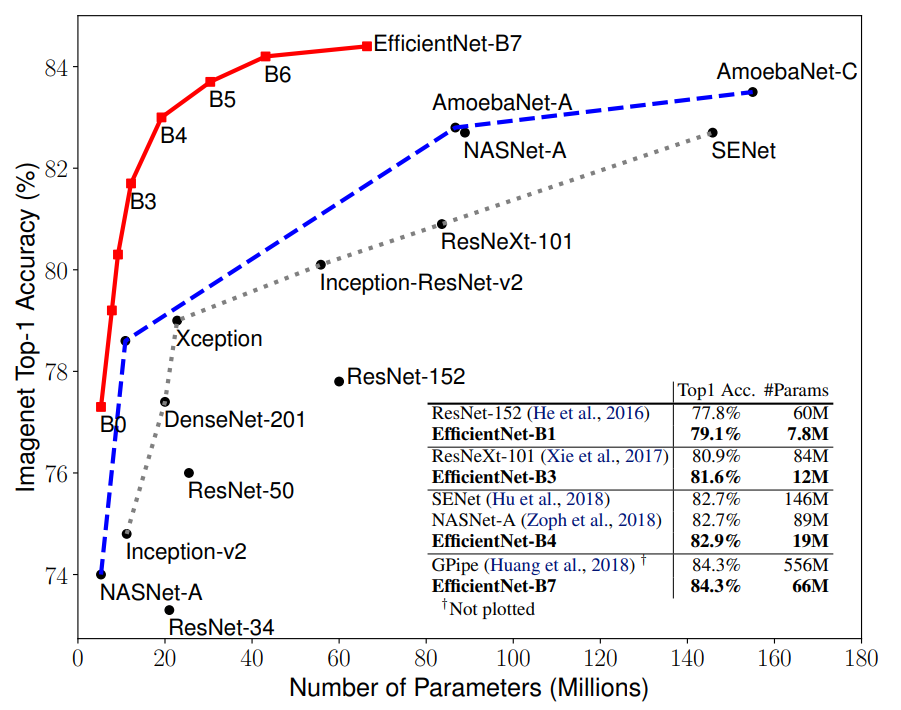
\includegraphics[scale=0.45]{Images/efficient-net-accuracy.png}
    \caption{Precision of EfficientNet compared to other known architectures~\cite{EfficientNet}.}
    \label{fig:efficientNet}
\end{figure}

As observed in Figure \ref{fig:efficientNet}, the \textit{EfficientNet} architecture outperforms other well-known network architectures in terms of accuracy on the \textit{ImageNet} dataset while maintaining a relatively low parameter count. The graph compares successive versions of the \textit{EfficientNet} network with other architectures that offer similar accuracy levels. It turns out that in every comparison, \textit{EfficientNet} operates with significantly fewer parameters. For instance, \textit{EfficientNet-B7} achieves the same accuracy as the \textit{GPipe} network but is described by more than 8 times fewer parameters, making it over 6 times faster.

\textit{EfficientNet} is built around the idea of strategic model scalability, which is achieved through adjustments in three key dimensions:
\begin{enumerate}
    \item Network \textbf{width} (the number of convolutional network filters)
    \item Network \textbf{depth} (the number of hidden layers)
    \item Input image \textbf{resolution}
\end{enumerate}

\begin{figure}[!htb]
    \centering
    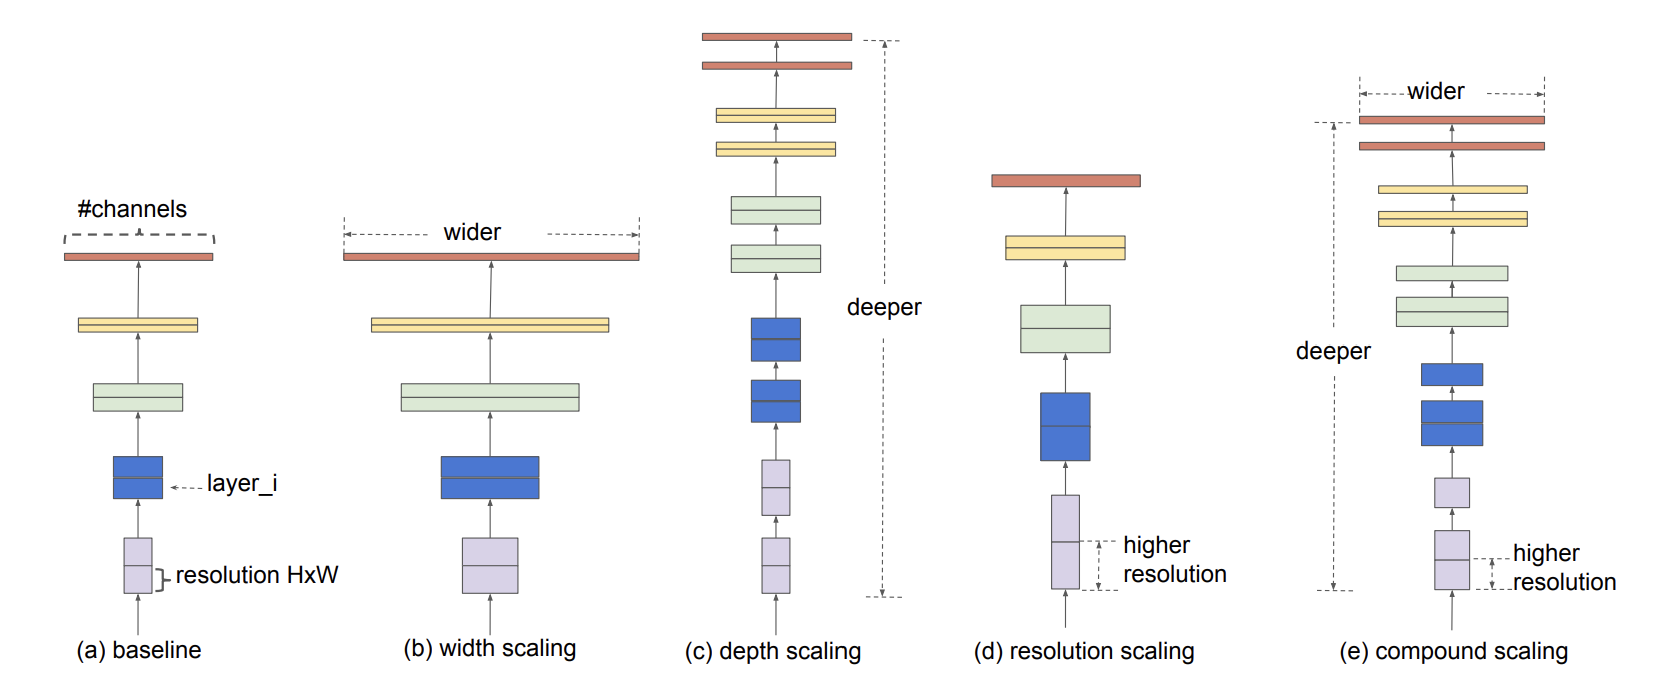
\includegraphics[scale=0.7]{Images/efficient-net-model-scaling.png}
    \caption{Model Scaling. (a) a baseline network example; (b)-(d) are conventional scaling - one dimension of a network at a time: width, depth, or resolution. (e) compound scaling method that scales all three dimensions with some fixed ratio~\cite{EfficientNet}.}
    \label{fig:modelScaling}
\end{figure}

This concept is illustrated in Figure \ref{fig:modelScaling}. The authors observed that scaling the network in \textbf{all dimensions simultaneously} yields the best results and proposed a novel approach known as the \textbf{compound scaling} method, which utilizes a parameter denoted by $\phi$, as follows:

\begin{equation}
    \begin{cases}
      depth: d = \alpha^\phi\\
      width: w = \beta^\phi\\
      resolution: r = \gamma^\phi
    \end{cases}\,
    \label{eqs:scaling}
\end{equation}

Under the assumptions that $\alpha \cdot \beta^2 \cdot \gamma^2 \approx 2$ and $\alpha \geq 1$, $\beta \geq 1$, $\gamma \geq 1$, where $\alpha$, $\beta$, and $\gamma$ can be determined through a manual grid search of small value sets. Intuitively, $\phi$ represents a parameter that signifies the amount of computational resources available for allocation, while the parameters $\alpha$, $\beta$, and $\gamma$ dictate how these resources are distributed across each dimension.

To significantly improve network performance using the scaling method described above, it is also essential that the foundational architecture (\ref{fig:modelScaling}) is appropriate. To create the EfficientNet, the authors specified a base architecture primarily composed of \textbf{mobile inverted bottleneck modules} (Figure \ref{fig:efficientNetBasicModel}). Then, they refined its architecture through the following steps:
\begin{enumerate}
    \item \textbf{Step 1}: They set the parameter $\phi = 1$, assuming the availability of double the computational resources, and carried out a grid search for the parameters $\alpha$, $\beta$, and $\gamma$. This process identified the most optimal values for these parameters within the base model as 1.2, 1.1, 1.15, under the constraint $\alpha \cdot \beta^2 \cdot \gamma^2 \approx 2$.
    \item \textbf{Step 2}: The parameters $\alpha$, $\beta$, and $\gamma$ were kept constant, and the base network was scaled using different values of $\phi$, following the scaling equation \ref{eqs:scaling}.
\end{enumerate}

\begin{figure}[!htb]
    \centering
    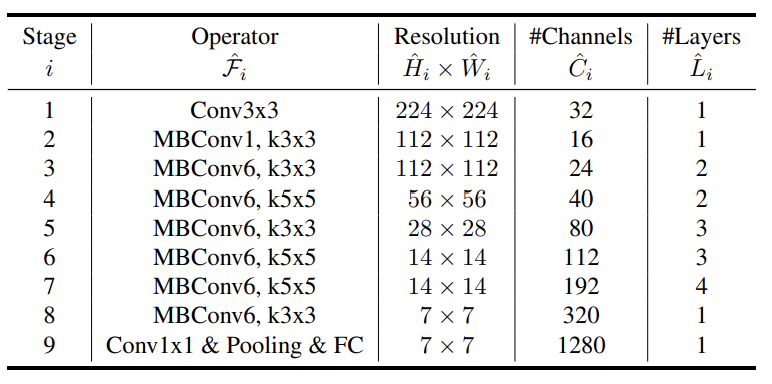
\includegraphics[scale=1]{Images/efficient-net-base-model.png}
    \caption{Baseline models used in \textit{EfficientNet}~\cite{EfficientNet}.}
    \label{fig:efficientNetBasicModel}
\end{figure}

The authors used saliency maps to assess the performance of the trained models. They found that scaling the dimensions of the network in each dimension separately improved the performance of the network, but the scaling method used in EfficientNets resulted in networks focusing on the most important parts of the input image during classification.